%#!make IN201503.dvi
\documentclass[technicalreport]{ieicej}
\usepackage[dvipdfmx]{graphicx}
% For URL support
\usepackage{url}


%======================================================================
% プリアンブル
%======================================================================
% 表示位置の修正
\hoffset -8mm
\voffset -8mm

%% 行間
\def\baselinestretch{0.95}

% ハイフネーションを修正
\hyphenation{net-works}

% 縦に並べた図の間の基準となるスペース
\newlength\figuresep
\setlength{\figuresep}{0.3\floatsep}

% enumerate環境のインデントを変更
\makeatletter
\renewenvironment{enumerate}
  {%
   \ifnum \@enumdepth >3\relax\@toodeep\else
    \advance\@enumdepth\@ne
    \edef\@enumctr{enum\romannumeral\the\@enumdepth}%
    \list{\csname label\@enumctr\endcsname}{%
    \leftmargin1.5zw
    \labelsep1zw
    \labelwidth\z@
    \itemindent2zw
    \listparindent1zw
    \topsep\z@\parsep\z@\partopsep\z@\itemsep\z@
    \usecounter{\@enumctr}%
    \def\makelabel##1{\hss\llap{##1}}}%
   \fi}{\endlist}
\makeatother

%----------------------------------------------------------------------
% タイトル
%----------------------------------------------------------------------
%和文タイトル
\jtitle{WLANとZigBeeの共存に向けたAP-Assisted CTS-Blockingの評価}
%英文タイトル
\etitle{Evaluation of an AP-Assisted CTS-Blocking aiming at co-existence of WLAN and ZigBee}

%著者たち
%E-mail掲載希望の場合は[ ]に含める
\authorlist{
 \authorentry{佐伯 良光}{Yoshiteru Saeki}{Kyu}
 \authorentry{石田 繁巳}{Shigemi Ishida}{Kyu}
 \authorentry{田頭 茂明}{Shigeaki Tagashira}{Kan}
 \authorentry{福田 晃}{Akira Fukuda}{Kyu}
}
\affiliate[Kyu]%
{九州大学大学院システム情報科学府・研究院 〒819--0395 福岡市西区元岡744番地}%
{Guraduate School/Faculty of Information Science and Electrical Engineering,
Kyushu University%
%Motooka 744, Nishi-ku, Fukuoka,
%819--0395 Japan
}
\affiliate[Kan]%
{関西大学総合情報学部 〒569--1095 大阪府高槻市霊仙寺町2-1-1}%
{Faculty of Informatics, 
Kansai University%
%2-1-1 Ryozenji-cho, Takatsuki-shi, OSAKA,
%569--1095 Japan
}

%======================================================================
% テキスト開始
%======================================================================
\begin{document}

%----------------------------------------------------------------------
% 和文あらまし
%----------------------------------------------------------------------
% 500字程度
\begin{jabstract}
 筆者らは,同周波数帯を利用するWLANとZigBeeの同空間における共存に向けて容易に構
 築可能な衝突回避システムの研究を行っている.
 衝突回避システムにおいては通信の公平性確保の為,システム改変に多くの制約がある.
 このような観点から,既存の方式を活用する,フレームを二重に送信する等,システム改変の
 制約にあたらないシンプルなシステム構築が重要となる.
 本稿ではZigBeeネットワークが無線LAN(WLAN)から受ける干渉の影響を軽減するための
 AP-Assisted CTS-Blocking(AA CTS-Blocking)を示す.
 AA CTS-BlockingはRTS/CTS方式を応用することでWLANの通信を抑制し,ZigBee通信と
 WLAN通信の衝突を回避させる.
 AA CTS-Blockingを用いた干渉回避システムを実装し,実証評価を通じてZigBeeネットワーク
 の通信エラー率を評価する.
\end{jabstract}

%和文キーワード
\begin{jkeyword}
 WLAN,ZigBee,干渉回避,AA CTS-Blocking.
\end{jkeyword}

%----------------------------------------------------------------------
% 英文あらまし
%----------------------------------------------------------------------
% 100 words程度
\begin{eabstract}
 The authors readily configured toward the coexistence in the same space of the WLAN and ZigBee utilizing the same frequency band
 You are conducting research on dating possible collision avoidance system .
 Because in the collision avoidance system of fairness ensure communication , there are a number of constraints on the system modification .
 Etc. from this point of view , to use the existing access control system , to double the header packet ,
 Simple system construction that does not hit the constraint is important .
 This paper is to reduce the effects of interference ZigBee network receives from a wireless LAN (WLAN) is
 AP-Assisted CTS-Blocking I show the (AA CTS-Blocking).
 AA CTS-Blocking inhibits communication of the WLAN by applying the RTS / CTS method , a ZigBee communication
 I to avoid the collision of WLAN communication .
 Implements the collision avoidance system using AA CTS-Blocking, and ZigBee network through empirical evaluation
 I evaluate the communication error rate .
\end{eabstract}

%英文キーワード
\begin{ekeyword}
 Wireless-Local Area Network (WLAN),ZigBee,Collision Avoidance,Access Point-Assisted 
 Clear to Send-Blocking (AA CTS-Blocking)
\end{ekeyword}

\maketitle

%======================================================================
% 本文ここから
%======================================================================
\section{はじめに}
\label{sec:intro}

%近年,複数のセンサ付無線端末を空間に散在させ,それらが協調して環境や
%物理的状況を採取する無線センサネットワーク(Wireless Sensor Networks, 
%WSN)が注目を浴びている.

%現代社会において,無線通信ほど一般化しているものはない.

現代社会において,無線ネットワークによる通信は生活に不可欠な存在である.
特に近年は,スマートフォンの登場によりWi-fiに代表される
無線LAN(Wireless LAN,WLAN)通信は広く一般に普及している.
%例えばPCとプリンタを,自宅の無線LAN(Wireless LAN,WLAN)の
%アクセスポイント(Access Point,AP)に接続して印刷を行うことは珍しくない.
%それだけにとどまらず,更にHDD,テレビ,レコーダーなど,様々なデジタル機器を
%WLANネットワークに接続して利用するホームネットワークという概念も登場している.
%近年では,WLAN通信端末の主体がスマートフォンやタブレットで代表される
%モバイルワイヤレス端末に移行しつつある.
%コンビニエンスストアや駅など,不特定多数の人々がゲストとしてアクセス可能な
%WLAN APの設置も進んでいる.
%特定の場所に限らず,あらゆる地域・場所でWLANネットワークに
%接続して通信することが求められるようになってきている.
%このように,WLANネットワークによる通信は広く一般に普及している.
他方で,別のネットワーク通信としてZigBeeが注目されている.
%ZigBeeとは,センサーネットワークを主目的とする近距離無線通信規格の1つであり,
ZigBeeはIEEE 802.15.4に準拠した規格であり,WLANに比べ通信距離が短く
通信速度も低速であるが,安価で省電力である.
それ故に,ネットワークに繋がれた機器同士が人間を介在せずに通信し,
サービスを提供するM2M(Machine to Machine)技術によく利用される.
M2Mの応用範囲は非常に幅広く,多様なサービスを提供可能である.
屋内にZigBeeネットワーク接続されたセンサを配置して,
電力やガスの消費量や,温度を最適に自動制御するスマートハウスもM2Mの1つである.
%↑農業の話に変えるか

ネットワーク技術の進歩に伴い人々の暮らしが益々便利になる
一方で,通信フレームの衝突による干渉という課題も存在する.
例えば,ZigBeeセンサにより構築されたスマートハウスを利用する場合,
屋内にWLAN APが存在すれば干渉が発生する可能性は高い.
%(修論で)干渉とは,電波技術Aに対応した受信機Txが電波Aと電波Bの混在した電波を受信した際,正常に電波をデコードできないことを指す.
それはZigBeeが,WLANと同じ2.4GHz帯を利用するためである.
図\ref{fig:frequency}に,WLAN及びZigBeeの周波数チャネルを示す.
ZigBeeとWLANの中心周波数が近いところでは,相互に干渉が生じる~\cite{Shuaib06:}.
WLANはZigBeeに比べて10〜100倍程度送信電力が大きい~\cite{Chieh10:}ため,
干渉による通信への影響はZigBee側が大きい.
%干渉は通信フレームの衝突により発生する.
%2.4GHz帯のZigBee及びWLANの周波数チャネルを図1に示す.
%ZigBeeでは,11chから26chの合計16チャネルに分割している.
%WLANでは,1chから13chまでの合計13chに分割している.
%ZigBeeとWLANのチャネルにおいて,オーバーラップしていない
%チャネルは存在しない.

\begin{figure}[bt]
 \centering
 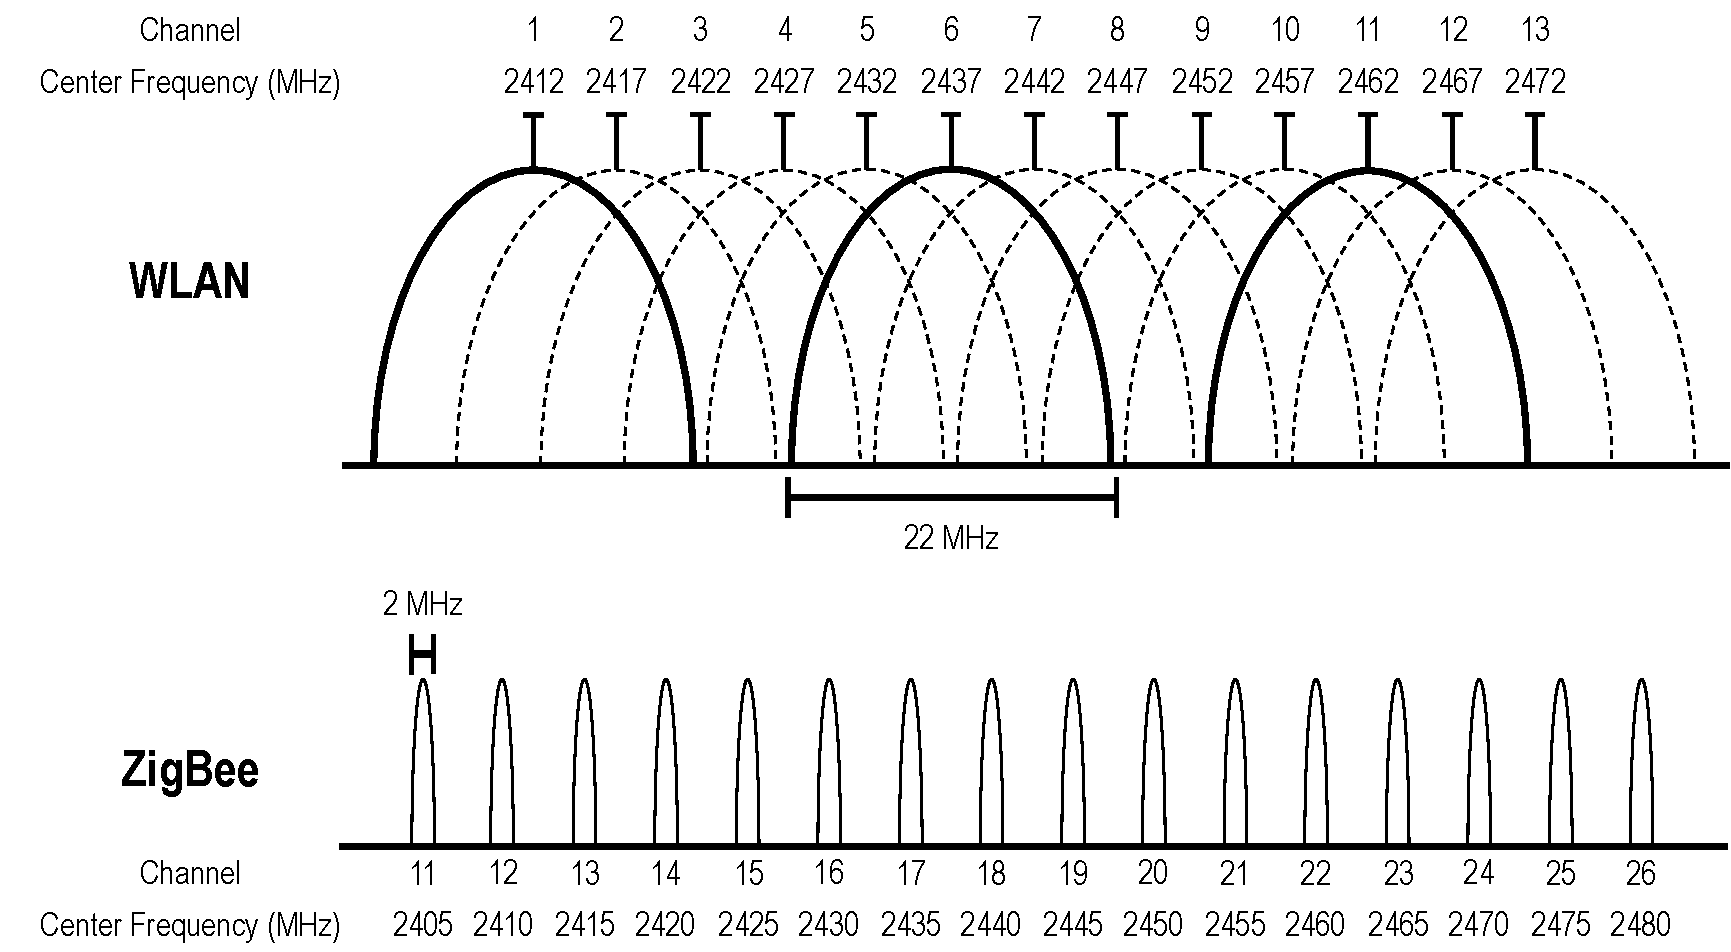
\includegraphics[width=\columnwidth]{figure/frequency.pdf}
 \caption{WLAN及びZigBeeの周波数チャネル}
 \label{fig:frequency}
\end{figure}

WLAN,ZigBeeにはアクセス制御方式としてCSMA/CA
(Carrier Sense Multiple Access / Collision Avoidance)機構を具備している.
しかし,WLANのCSMA/CAではWLANのみの通信環境,
ZigBeeのCSMA/CAではZigBeeのみの通信環境を想定しているため,
%これはWLANのみの通信環境,もしくはZigBeeのみの通信環境を想定しているため,
%従って,同種の通信における干渉回避を目的としている.%←合ってる?
%そのため,異種の通信におけるフレーム衝突回避を目的とした
WLAN通信とZigBee通信が混在した環境における複数モジュールの制御は困難である.

同環境内におけるWLANとZigBeeの共存を目的とした干渉回避方式として,
文献~\cite{Hou09:}ではWLANのアクセス制御であるRTS/CTS(Request to Send / Clear to Send)方式
を利用したCTS-Blockingが提案されている.
図\ref{fig:cts_blocking}に,CTS-Blockingの概要を示す.
CTS-Blockingでは,制御PCからCTSフレームを直接送信することで周囲の
WLAN端末の通信を一時的にブロックする.
WLAN通信において,送信端末以外の端末がCTSフレームを受信すると
CTSフレーム内の\texttt{Duration}フィールドに記載された時間だけ送信を控える.
CTS-Blockingではこれを利用して周囲のWLAN端末の
通信を抑制し,WLANとZigBeeの干渉を回避する.
しかしながら,現在のOS・無線LANモジュールでは通信の公平性確保の観点からCTS
フレームの直接送信が禁止されており,CTS-Blockingの実現に向けてハードウェアや
OSの改変が必須となるために実現が難しい.
また,送信電力制御の影響によりCTSフレームの到達範囲が狭くなる可能性があり,隠れ端末問題の影響を受けやすい.

WLANとZigBeeの共存のためには,%WLANのアクセス制御を行うことで
干渉されないZigBee通信を容易に実現することが重要である.
筆者らは,既存のRTS/CTS方式をそのまま利用した
%WLANのアクセス制御である
AP-Assisted CTS-Blocking(AA CTS-Blocking)干渉回避方式の開発を進めている.
本稿では,AA CTS-Blockingの有効性の検証に向けた実証評価について報告する.

\begin{figure}[bt]
 \centering
 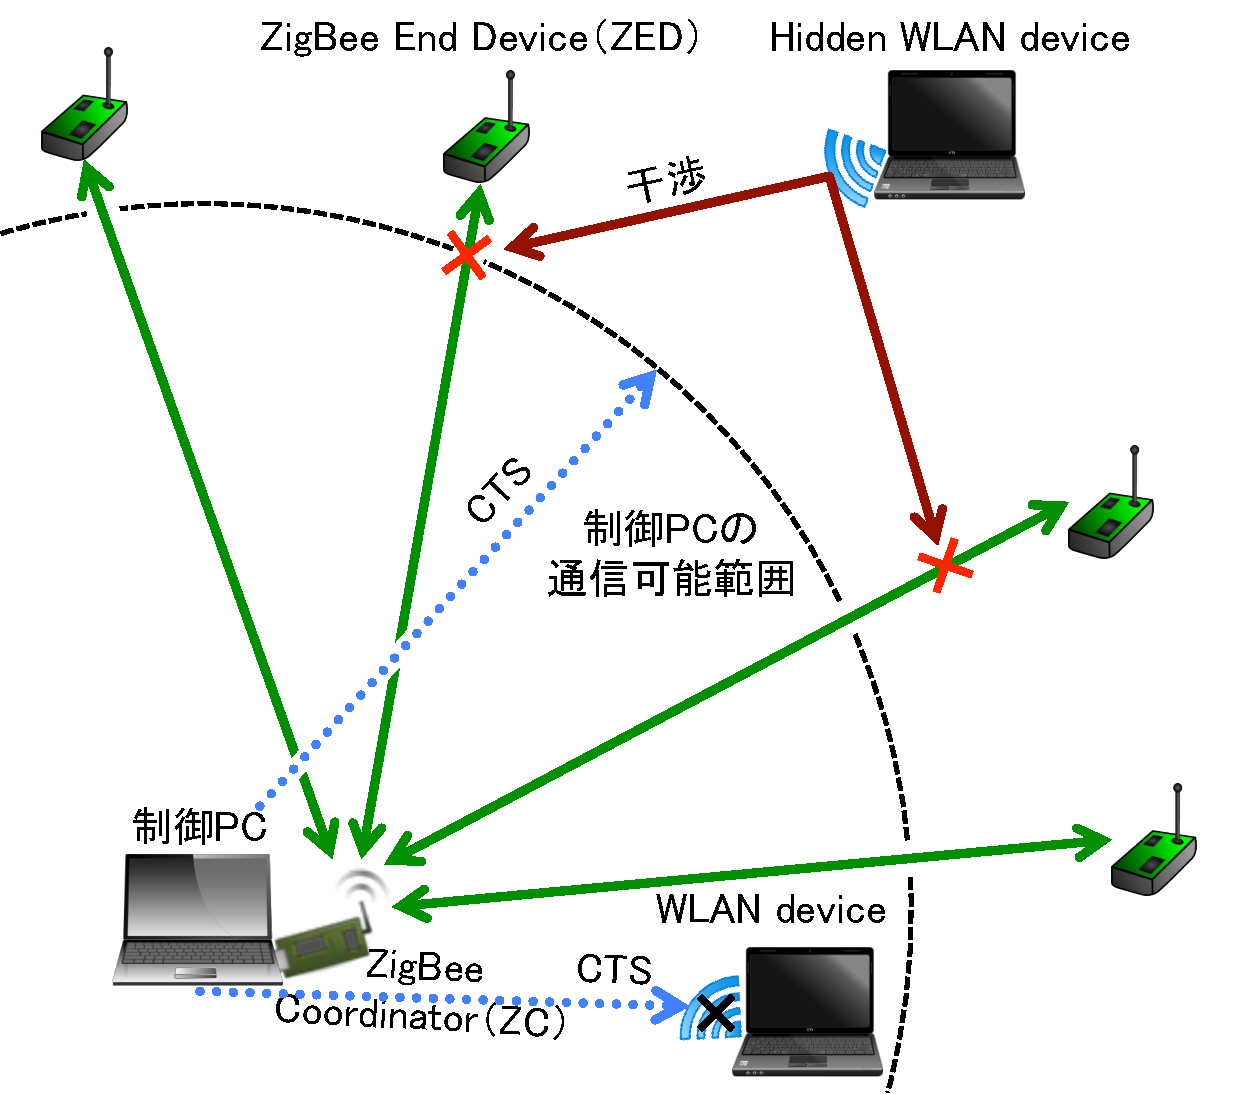
\includegraphics[width=\columnwidth]{figure/cts_blocking.pdf}
 \caption{CTS-Blockingと隠れ端末問題}
 \label{fig:cts_blocking}
\end{figure}

本稿の構成は以下の通りである.
\ref{sec:wlan_and_zigbee}ではWLANとZigBeeの共存に向けた干渉回避方式を提案する
関連研究について述べ,それぞれが提案するシステムの利点と欠点について述べる.
\ref{sec:aa_cts}では筆者らが提案するAA CTS-Blocking方式の概要及び設計について示す.
\ref{sec:imple}ではAA CTS-Blocking方式を適用した
ZigBeeノードによるデータ収集システムの実装について述べ,
\ref{sec:eval}でWLAN通信環境下におけるZigBeeノードによるデータ収集システムについて,
AA CTS-Blocking方式の有無による通信成功率の差を比較・考察する.
最後に\ref{sec:conclu}でまとめとする.

%SNWその1
%センサネットワークの構想は戦闘地域の監視など軍事目的に端を発するが,
%現在は民生用途,特に省エネルギー管理、工業計装、居住環境、自然保護、健康管理、交通状況などのモニタを目的とするものが多い。搭載するセンサの種類および入力形式は電力・温度・湿度・ガス・照度、アナログ・EIA-485・Modbusなど種類、形式を問わない。
%センサネットワークの無線端末はノードと呼ばれ、通常1個以上のセンサ、無線チップ、マイクロプロセッサ、電源(電池など)により構成される。当初構想では粒のように小さく作り、意識されずして遍在する、というユビキタス構想を目標としていたため「モート(Mote、塵)」や「スマートダスト(賢い埃)」などの呼称で研究開発が進んだ。しかし実際には電池の容積に依存すること、塵ほど小さくする必要がない、などの理由で大きさより機能重視で開発されるものが大半となった。

%SNWその2
%センサネットワークは通常、アドホック(ad hoc)機能と、各ノードから中枢ノードへデータを送るためのルーティング機能(routing algorithm)を持つ。つまり、ノード間の通信に障害がでると別の通信経路を自律的に再構築する機能がある。ノードがグループとして連携するため分散処理の要素もある。加えて、外部から電力供給を受けずに長期間動作する機能もあり、そのために省電力機能または自己発電機能を持つ。
%上記を達成するための技術として、無線、ネットワーク、MEMSセンサ、センサインターフェース、電池(または自己発電)、およびそれらの信頼性を損なわずに実働温度範囲で長期間動作させる方法など、広い裾野分野の連携が必要とされる。

%IoTについて
%近年,さまざまなモノがインターネットに接続している状態を指す
%IoT(インターネット・オブ・シングス)という言葉が登場した.
%2009年にはインターネットに接続するモノの数は約25億個であったのが,
%2020年には260億個を超えると推測されている.
%IoTはIT分野に限らず,今後あらゆる産業分野で広がっていくと考えられる.

%ユビキタスネットワーク(SNW?)についてまとめ
%近年,高速な通信サービスを提供するブロードバンドネットワークに加えて,
%無線ネットワーク技術を応用した「いつでも・どこでも・誰とでも」情報の
%やりとりが可能となる「ユビキタスネットワーク」の研究が加速している.
%今後,無線通信機能を備えた多数の小型センサーが身の回りの至るところで
%自律的にネットワークを構成し,サービスを提供するような大規模なセンサ
%ーネットワーク(ユビキタス・センサーネットワークとも呼ばれる)の実現
%が注目されている.
%センサーネットワークでは,多数かつ多様なセンサーが広範囲に接続され,
%これらの個々のセンサーから収集される膨大な情報を適切に処理し,人・
%モノの状況やそれらの周辺環境を的確に認識し,その状況に即した最適な
%動作を自律的に行うシステムを構築する必要がある.


%例えば,農業分野ではZigBeeノードを利用したセンサネットワークの活用,
%自動車産業分野では運転支援システムといった様に,
%それほどまでに,現代社会は無線ネットワークが発達し,浸透している.
%人々の暮らしがより便利になる一方で,解決すべき課題も見えてきた.
%その一つに,通信における干渉がある.
%そもそも無線通信サービスを提供する通信事業者や放送局などは,
%それぞれ総務省から割り当てられた周波数帯で電波を送出している.
%これは多様な電波を効率よく共存させる目的で,利用できる範囲を振り分けているため,
%干渉による影響を受けにくい.
%しかしISMバンドという,本来は無線通信以外の利用用途で割り当てられた2.4GHz帯で
%普及してきた無線LANやZigBeeなどは事情が違う.
%異なる無線アクセス技術にも関わらず使用する周波数帯が重なるため,干渉によって
%通信速度の低下などの影響を受ける.
%特にZigBeeに比して無線LANの送信電力は10~100倍と大きいため,ZigBeeへの影響が顕著である.

%様々なネットワークについて
%近年,%携帯電話,PHS,Wi-FiおよびBluetoothなど
%多様な無線システムの利用拡大が進んできている.
%さらに,IEEE802.16の標準規格も進み,WiMAXやMobile WiMAX
%による広域または中域の高速無線システムの利用も予想される.
%このように,無線システムは急速に利用拡大と多様化が進み,
%無線通信環境は異なる周波数帯域や通信方式を持つ多様な無線システムが混在する環境となりつつある.

%WLANについて
%インターネットのインフラ化に伴い,あらゆる地域・場所で
%ネットワークに接続することが求められるようになってきた.
%また,リッチコンテンツの増加や動画などマルチメディア通信
%の増加などからブロードバンド通信が強く求められてきている.
%さらに,通信端末の主体がスマートフォンやタブレットで代表さ
%れるモバイルワイヤレス端末に移行しつつある.このような社
%会的背景から,移動体ブロードバンド通信技術への期待が高まっ
%ている.これまでの無線LAN技術は,AP(Access Point)と端末が
%一体となった移動アドホックネットワークにおいては,APが
%移動するということが考えられているが,
%それ以外では,端末は移動するが,APは固定であるという前
%提での議論が多かった.

%----------------------------------------------------------------------
\section{関連研究}
\label{sec:wlan_and_zigbee}

筆者らの調査の範囲では干渉回避方式に関する研究は膨大に存在するため,
本節ではそれらについて俯瞰する.

まず,WLANのアクセス制御方式,CSMA/CAを利用した干渉回避方式の提案について示す.
%CBT~\cite{Zhang11:},ACROS~\cite{Shin10:}においても同様の問題が考えられる.
CBT~\cite{Zhang11:}では,
%CBT(Co-operative Busy Tone)
CSMA/CAを用いて,WLAN端末にZigBee通信が開始されることを知らせ
ZigBeeノード間で通信が行われる間WLAN端末のデータ送信を控えさせ,
WLANとZigBeeのフレーム衝突を回避する.
しかしながら,
CBTシステムの構築には全WiFi端末の近くにsignalerと呼ばれるZigBeeノードを
配置する必要があるため,移動体WLAN端末に対して非現実的である.

別のWLANのアクセス制御方式であるDCF(Distributed Coordination Function)を利用した
干渉回避方式も提案されている.
村田ら~\cite{Murata14:}は干渉の原因をZigBeeのaTurnaroundTime(送受反転時間)が
通信アイドル時の待機時間であるDIFS(DCF Inter Frame Space)よりも長いことと捉え,
DIFSを拡大する方式を提案している.
DIFSをaTurnaroundTimeに比べ長くとることで衝突を回避する.
しかしながら,DIFSを拡大するためには予めAPにアクセスして設定しなければならず,
%またDCFの欠点である,物理的障壁が存在した場合の隠れ端末問題の影響を考えると
実現のためには周囲のAP全てを管理下に置かなければならない.

また,ZigBeeが準拠しているIEEE 802.15.4のビーコンモードを利用した
干渉回避方式も提案されている.
Dynamic GTS~\cite{Huang09:}では,ビーコンモードの1つである
ZigBeeノードにGuaranteed Time Slot(GTS)を割当て優先的に通信できる期間CFP(Contention Free Period)
を利用し,このCFPを拡大することで衝突を回避する.
CFPの拡大は,GTSを動的に配置しそのビーコンを検知したWLAN端末が
CTSフレームを送信することで達成可能である.
しかしながら,\ref{sec:intro}で示したCTS-Blockingと同様に,
ハードウェアやOSの改変が必須である点,
隠れ端末問題の影響を受けやすい点が問題である.
CACCA~\cite{Tytgat12:}においても同様の問題が考えられる.

さらに,無線通信の通信空き時間を有効活用して通信を行うための「White Space」技術
を応用した干渉回避方式が提案されている.
WISE~\cite{Huang10:}では,WLAN通信におけるWhite Spaceを予測し,そのWhite
Space内で通信が完了するようにZigBeeフレーム長の動的制御を行う.
例えば,WLAN通信の混雑時には予測されるWhite Spaceの長さは短くなるため,
ZigBeeノードにおいてデータを分割して送信する.
これにより,ZigBeeフレームがWLAN通信によって破壊される確率を低減させるこ
とが可能となる.
しかしながら,WLAN通信が混雑している時にはWLAN通信の空き時間が少ないため
にWhite Spaceの予測が外れ,通信が衝突する確率が高くなる.
Adaptive Interference-Aware Multi-Channel
Clustering Algorithm~\cite{Kang07:}においても同様の問題が考えられる.

上記の関連研究群は,既存の方式やモジュールの改造が必要である,
もしくは特別なハードウェア等の利用が必須であるなど,
干渉回避方式の構築コストについて考慮されていない.
既存の方式のみを利用した干渉回避方式に関する研究は報告が少なく,
筆者らの調査の範囲ではBuzzBuzz~\cite{Chieh10:}が該当する.
BuzzBuzzでは,WLANとZigBeeのフレーム衝突により通信が阻害される原因として
IEEE 802.15.4フレームのヘッダが破壊されることと捉え,
ヘッダを2重にして送信することでZigBeeのパケットロス率を減少させている.
これは,本稿で提案するAA CTS-Blocking方式とは違うアプローチで
ZigBeeの通信を保証しており,
%干渉回避方式として効果を上げている.
AA CTS-Blockingと組み合わせることでさらなる干渉回避効果が期待される.

%干渉回避方式に関する研究は膨大に存在するため,本節ではそれらについて俯瞰する.


%RTS/CTS方式を利用した干渉回避システムについても提案されている.
%図\ref{fig:cts_blocking}に,CTS-Blocking~\cite{Hou09:}の概要を示す.
%CTS-Blockingでは,制御PCからCTSフレームを直接送信することで周囲の
%WLAN端末の通信を一時的にブロックする.
%送信端末以外の端末がCTSフレームを受信すると,CTSフレーム内の\texttt{Duration}
%フィールドに記載された時間だけ送信を控える.
%CTS-Blockingではこれを利用して周囲のWLAN端末の通信を抑制し,WLANとZigBeeの
%干渉を回避する.
%この手法では単純にCTSフレームのみを利用しているため,
%WLAN通信の混雑度に左右されず,事前にAPへアクセスしてDIFSを設定する必要ない.
%これまで紹介してきた手法の中では,最も実環境における干渉回避効果が高いと期待できる.
%しかしながら,現在のOS・無線LANモジュールでは通信の公平性確保の観点からCTS
%フレームの直接送信が禁止されており,CTS-Blockingの実現に向けてハードウェアや
%OSの改変が必須となるために実現が難しい.
%また,送信電力制御の影響によりCTSフレームの到達範囲が狭くなる可能性があり,隠れ端末問題の影響を受けやすい.



%WLANとZigBeeの共存に向けて様々な手法,システムが提案されているが,
%その多くは複数のAPと自由なWLAN通信が行われる実環境に即していないように見受けられる.
%そこで筆者らは,実環境におけるWLAN及びZigBeeの干渉回避システムを目指し
%AP-Assisted CTS-Blockingを提案する.

%----------------------------------------------------------------------
\section{AP-Assisted CTS-Blocking}
\label{sec:aa_cts}

WLAN APは,WLAN端末に比べ送信電力が物理的に大きく,
RTS/CTS制御方式においても利用されるため,
これを利用して干渉回避方式であるAP-Assisted(AA)CTS-Blockingを提案する.
本節では,AA CTS-Blockingの概要を示し,
構築のための課題について検討する.

%APからCTSフレームを送信することはRTS/CTS制御方式において
%一般的であるため,OSやハードウェアの改変が不必要となる.
%またWLAN端末に比べ,WLAN APの送信電力が物理的に大きいことに着目し,
%AP-Assisted(AA)CTS-Blockingを提案する. 
%AA-CTS Blockingでは,周辺にあるWLAN APからCTSフレームを送信させてCTS-Blockingを実現する.
%かつ隠れ端末問題によるWLANフレーム衝突が改善され,ZigBee通信効率の向上が期待される.

\subsection{概要}
\label{ssec:outline}

%これにより,WLAN通信の一時的ブロックによる効率的なZigBee通信の実現を目指す.
%また,RTSを送信するAPの選択については,APから取得できる情報を基に最適なAP選択アルゴリズムを考慮する.
図\ref{fig:aa_cts_blocking}に,AA CTS-Blocking方式の概要を示す.
本システムは,環境内に配置された複数のZigBee End Device(ZED)及び
ZigBeeネットワーク制御を行うZigBee Coordinator(ZC),制御PCから構成される.
ZigBee基地局と制御PCは有線接続されている.
AA-CTS Blockingでは,周辺にあるWLAN APからCTSフレームを送信させることでWLAN通信をブロックし
干渉の影響を低減したZigBeeノード間の通信を実現する.

%ZigBeeの通信を開始する場合,周囲のAPの1つを選択して制御PCからRTSフレームを送信する.
%選択されたAPはRTSフレームを受信すると周囲のWLAN端末に対してCTSフレームを送信する.
%制御PCはAPからのCTSフレームを受信するとZCを用いて複数のZEDとの通信を開始する.
%WLAN APは,そのAPが提供するWLANネットワークに参加していない端末からのRTSフレームに対しても
%CTSフレームを返答するため,制御PCでは任意のAPを選択することができる.

\begin{figure}[bt]
 \centering
 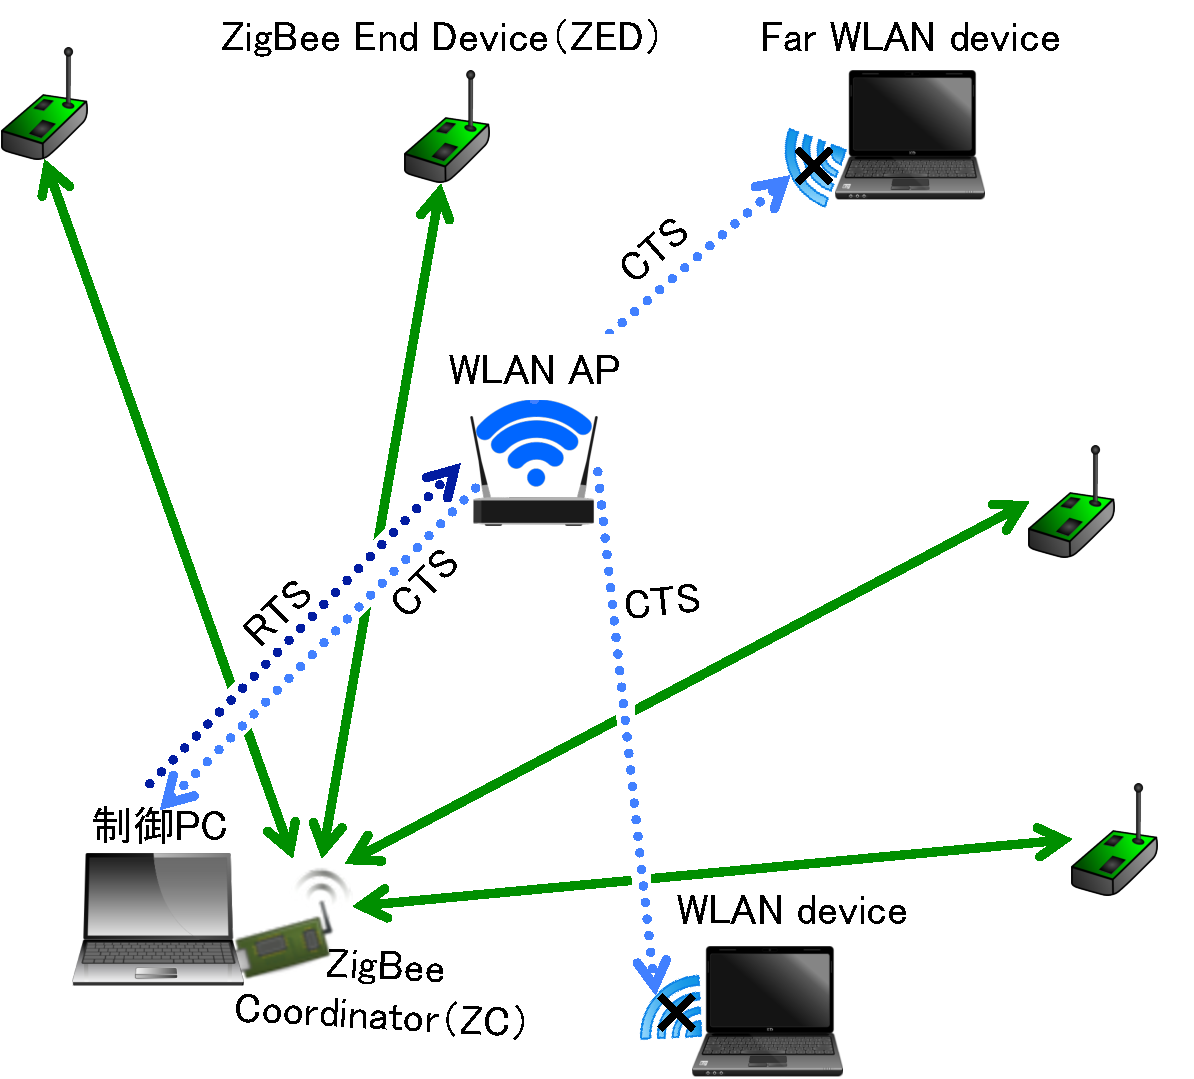
\includegraphics[width=\columnwidth]{figure/aa_cts_blocking.pdf}
 \caption{AA CTS-Blocking}
 \label{fig:aa_cts_blocking}
\end{figure}

\figurename~\ref{fig:sequence}にAA CTS-blocking方式を実現するための
通信シーケンスを示す.
制御PCは,予め周囲に存在するWLAN APのビーコンフレームを受信し,
チャネル,受信信号強度(RSSI)等を収集しておく.
ZigBeeノード間の通信を行う場合,まず(1)~制御PCはAPを1つ選択し,
(2)~制御PCは選択したAPに向けてRTSフレームを送信する.
次に(3)~RTSフレームを受信したAPは
周囲のWLAN端末に向けCTSフレームをブロードキャストする.
CTSフレームを受信したWLAN端末はCTSフレーム内の\texttt{Duration}
フィールドに記載された時間だけ送信を控えるため,WLAN通信が一時的にブロックされる.
WLAN通信ブロック期間がスタートした時,
(4)~CTSフレームを受信した制御PCは,有線接続されたZCに向けて通信開始信号を送信することで
ZigBeeノード間の通信を開始する準備が整う.
ZigBeeノード間の通信は,
ZCを用いた制御によりWLAN通信ブロック期間内に完了させる.

このようなAA CTS-Blockingを実現する上では2つの疑問が生じる.
\begin{enumerate}
 \item RTS送信先APをどのように選ぶか
 
	実環境には多くのWLAN APが存在するため,
	制御PCはRTSの送信先APを選択する必要がある.
	%APによるCTS-Blockingの効果は選択するAPによって大きく異なるため,重要である.
	\ref{ssec:select_ap}において,周囲に存在するWLAN APのビーコンフレームを用いた
	AP選択アルゴリズムを示す.

 \item WLAN通信ブロック期間において,ZigBeeノード間通信をどのようにスケジューリングするか
 
 	WLAN通信ブロック期間は有限であるため,
	%ZEDの数が多いほど通信回数が増え,時間的制約が厳しくなる.
	%ZigBeeノード間通信が増加しても,
	ZigBeeノード間で通信の衝突が起きないようアクセス制御を行う必要がある.
	%データ収集のZigBeeネットワークでは,ZCと複数のZEDによるスター型のネットワークトポロジーになる.
	%ZigBeeノード間通信でフレーム衝突が起きないよう,スケジューリングを行う必要がある.
	%AA CTS-BlockingではZigBee通信成功率の向上を目的としているので,
	%WLANとZigBeeの干渉以外の事象に起因する通信失敗率の値を排除した
	%AA CTS-Blockingによる純粋なZigBee通信成功率の向上値を示すためにも重要である.
	\ref{ssec:design}において,1台のZCと複数のZEDとの通信における
	スケジューリング手法を検討する.

\end{enumerate}

\begin{figure}[bt]
 \centering
 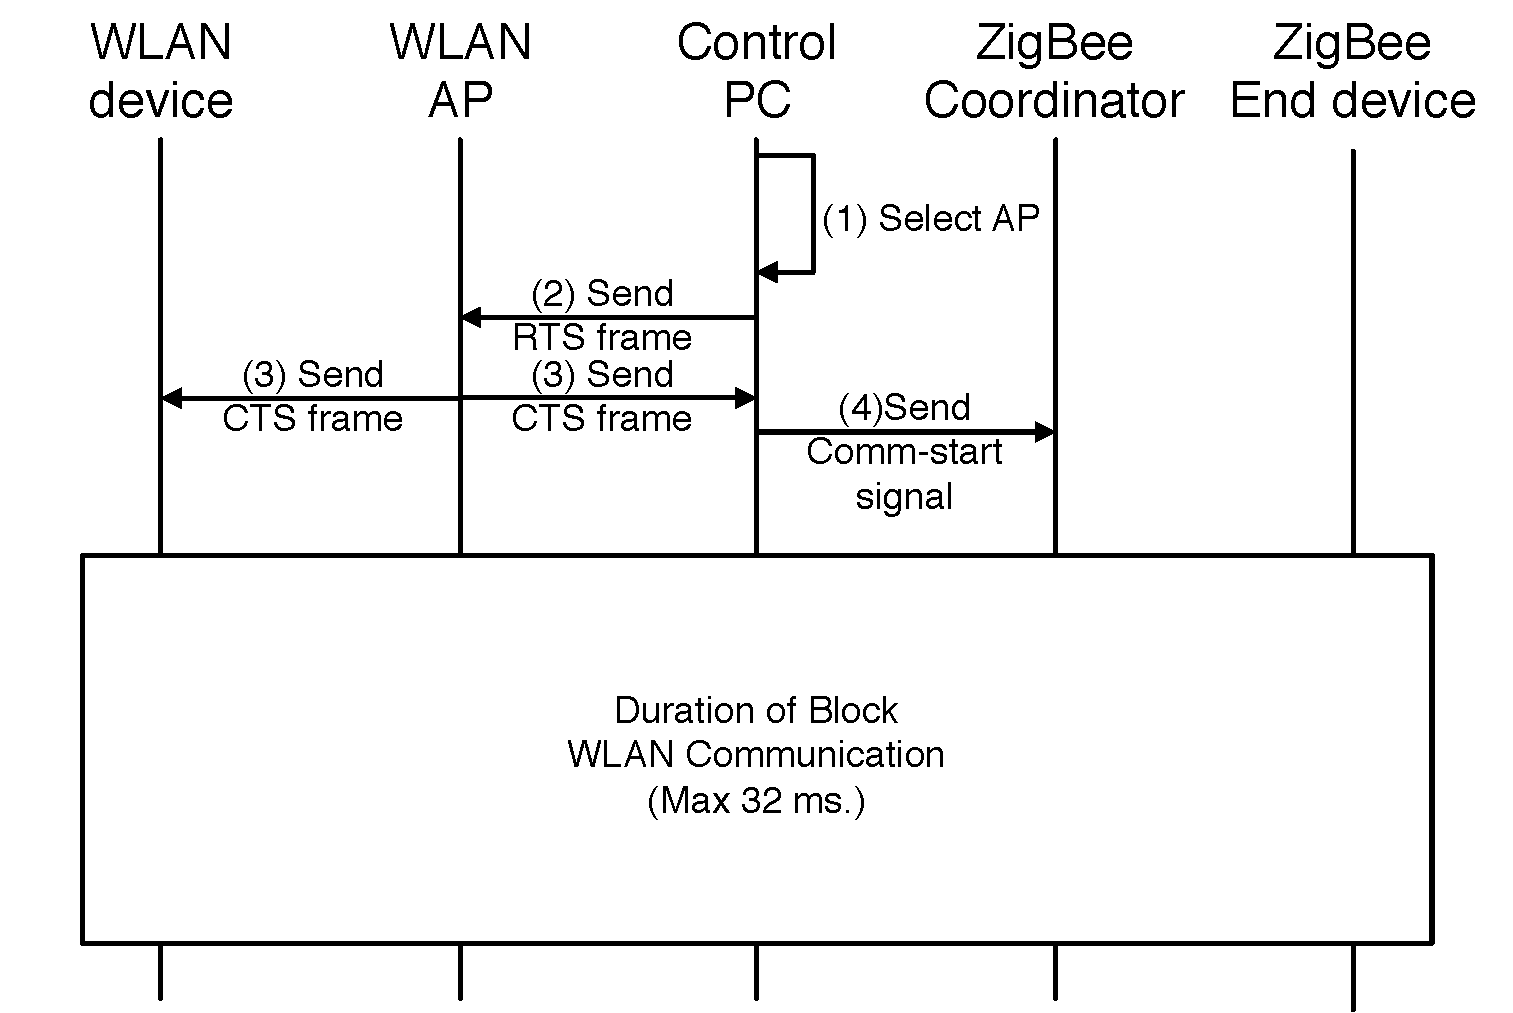
\includegraphics[width=\columnwidth]{figure/sequence.pdf}
 \caption{AA CTS-blocking方式の通信シーケンス}
 \label{fig:sequence}
\end{figure}

\subsection{AP選択アルゴリズム}
\label{ssec:select_ap}

AA CTS-Blockingにおいては,RTSフレームの送信先APの選択は
干渉回避性能に大きな影響を及ぼす.
例えば,制御PCの通信可能範囲内にないAPを選択した場合
RTSフレームが届かないため無意味である.
%↓ここは情報が足りない
%あまり通信を行っていないAPを選択した場合
%わずかなWLAN端末の通信しかブロックできず本システムによる効果が薄い.
RTSフレーム送信先APの選択を最適化することにより,
より多くのWLAN通信をブロックできる.
%× なぜならば,RTSフレームが制御PCの通信可能範囲にある必要がある
%○ 淡々と述べる
%制御PCとZCは一体になっている
%→データ収集システムにおいて,ZEDはZCを中心に周囲に配置されたものだとすると,
%RSSIによるWLAN通信のブロックはものすごく有効
APと制御PCの物理的距離が重要になると考え,
位置推定~\cite{izumi13:}などにも用いられる
RSSIをAP選択アルゴリズムのキーとして採用した.
RSSIの取得は特殊なパラメータや追加のデバイスを必要とせず,
%AP選択アルゴリズムに使用できる情報は,
既存のAPから発せられるWLANフレームから収集可能である.
図\ref{fig:aa_cts_blocking}に示すように制御PCがZCに有線接続されており,
ZEDはZCを中心に周囲に配置されていることも考慮に入れると,
制御PC周辺のWLAN通信をブロックすることが非常に有効であると考えられる.
%最も近いAPを選択することは非常に有効である.
%RSSIによるWLAN通信のブロックはものすごく有効
%ここで,本システムが有効であるためには
%制御PCの通信可能範囲にAPが存在する必要がある.
%従って,APと制御PCの物理的距離が重要になると考えられるため
%位置推定~\cite{izumi13:}などにも用いられるRSSIをAP選択アルゴリズムのキーとして採用した.
%具体的には,RTSフレームの送信先APとしてRSSIがもっとも大きいAPを
%選択するものとした.

\subsection{スケジューリング手法}
\label{ssec:design}

%APから周囲のWLAN端末にCTSフレームが送信されると,
%ブロック時間はCTSフレーム内の\texttt{Duration}フィールドに記載された時間に等しい.
%マルチキャストなZigBeeノード間通信において,フレーム衝突を防ぐための
%スケジューリングは重要である.
AA CTS-Blocking方式においては,ZigBeeノード間通信はAPから送信されたCTSフレーム内の
\texttt{Duration}フィールド(最大値は32\,ms~\cite{Bellardo09:})に記載された時間内に終了させる
必要がある.
ZEDの台数が増えた場合通信回数が増え,1キャストあたりの制約が厳しくなるため,
スケジューリング等のアクセス制御方式がなければフレーム衝突等が起こりやすくなる.

しかし,既存のMACプロトコルを利用すればこの問題は解決する.
32\,ms~程度ではあるが一定の通信時間を確保できるためである.
ZEDの台数が32\,ms間で通信できない台数に増加した場合においても,
各ZEDにノード番号を与え通信タイミングを制御することで
フレーム衝突は大幅に減少すると考えられる.
このスケジューリングに関しては,
MACプロトコルの種類は問わず,どの手法でも適用可能である.

%AA CTS-Blocking方式ではZigBeeノードを用いたデータ収集システムへの適用を想定しており,
%使用環境としてはWLANとZigBeeの干渉による影響が大きい,
%利用周波数帯の変わらない状況を想定している.
%\figurename~\ref{fig:star}に示す代表的なZigBeeネットワークトポロジーの中で最も低コストな,
%ZC1台にZED複数台をそれぞれ1対1で接続するスター型を採用すると考えると,
%ZCからZED方向の送信はブロードキャストであり,ZEDからZC方向の通信はシングルキャストとなる.
%シングルキャストでは,ZCに向けた異なるZEDからの
%データフレーム衝突を回避するスケジューリングが必要であるが.
%これはTDMA(Time Division Multiple Access,時分割多元接続)で十分である.

一例として,TDMA(Time Division Multiple Access)方式のMACプロトコルを利用する場合,
\ref{ssec:outline}で示したZigBeeノード間の通信シーケンス部分は以下のようにすれば良い.
通信開始信号を検出したZCは,周囲のZEDへデータ要求フレームをブロードキャストする.
%各ZEDはTDMA方式に従うので,
データ要求フレームを受け取ったZEDは,ZED毎に定められたSlot Sizeの時間だけ待機する.
Slot Sizeの時間が経過した後,ZEDはZCへデータフレームを送信する.

%AA CTS-blocking方式全体の通信シーケンスとして,\ref{ssec:outline}からの続きを考えることにする.
%例えば,スケジューリングとしてTDMA(Time Division Multiple Access,時分割多元接続)方式を利用した場合
%Zigbeeノード間の通信シーケンス部分は以下の様になる.
%(5)~通信開始信号を検出したZCは,周囲のZEDへデータ要求フレームをブロードキャストする.
%各ZEDはTDMA方式に従うので,
%(6)~データ要求フレームを受け取ったZEDは,ZED毎に固定されたスロットサイズの時間だけ待機する.
%スロットサイズの時間が経過した後,
%(7)~ZEDはZCへデータフレームを送信する.

%この様にすることで,WLANネットワーク環境下においても
%AA CTS-BlockingによるZigBeeデータ収集システムは実現可能である.

%----------------------------------------------------------------------
\section{実装}
\label{sec:imple}

AA CTS-Blocking方式の動作の実証と基本性能の評価に向け,
PC及びZigBeeノード用いて,AA CTS-Blockingを適用した
ZigBeeノードによるデータ収集システムを実装した.
データ収集システムの概要を図\ref{fig:aacts_snw}に示す.
本システムでは,
代表的なZigBeeネットワークトポロジーの中でも最も低コストな,スター型を採用した.
ZEDのスケジューリングとしてTDMA方式を採用し,各ZED毎に定められたTime Slotを設けた.
Time SlotはZEDのNode IDと対応付けており,
最大のTime SlotでもWLAN通信ブロック期間を超えないように定めた.
%ZC及びZEDには予めNode IDを設定しておく.
%ZCのNode IDはZEDの送信先アドレス,
%ZEDのNode IDはTime Slotに対応付けている.
以下にデータ収集システムの動作を示す.
%\ref{ssec:outline}で示した通り,
通信開始信号を検出したZCは,周囲のZEDに向けてBoradCast Frame(BF)を送信する.
BFを受信したZEDは,BFをSlot同期信号として
ZED毎に定められたTime Slotに従い,Slot Sizeの時間だけ待機する.
Slot Sizeの時間が経過した後,ZEDはZCのNode IDを送信先アドレスとして
Unicast Frame(UF)を送信する.
%ZCが各ZEDへBFを送信することで通信を開始し,
%各ZEDがZCへUFを送信することでデータ収集が実施される.
%,待機後にZCへ送信した.
%Time SlotのSlot SizeはNode IDに比例する様に設定した.
%また,ZCのデータ収集実施時間はWLAN通信ブロック期間に等しく,
%この間は常に受信待機状態となるようにした.

ZC及びZEDに用いたZigBeeノードは日本国内で入手しやすく,センサノードとして一般的な
Crossbow社のMICAz MPR2600J~\cite{Device:}を用いた.
%MICAzにはNode IDが設定できる.
%AA CTS-Blocking方式ではZigBeeノードを用いたデータ収集システムへの適用を想定しており,
%使用環境としてはWLANとZigBeeの干渉による影響が大きい,
%利用周波数帯の変わらない状況を想定している.
%\figurename~\ref{fig:star}に示す代表的なZigBeeネットワークトポロジーの中で最も低コストな,
%ZC1台にZED複数台をそれぞれ1対1で接続するスター型を採用すると考えると,
%ZCからZED方向の送信はブロードキャストであり,ZEDからZC方向の通信はシングルキャストとなる.
%シングルキャストでは,ZCに向けた異なるZEDからの
%データフレーム衝突を回避するスケジューリングが必要であるが.
%これはTDMA(Time Division Multiple Access,時分割多元接続)で十分である.
%上記データ収集システムのノード
MICAzへの実装には,センサネットワークノード向けのイベント駆動OSとして
オープンソースで開発されているTinyOSを用いた.


\begin{figure}[bt]
 \centering
 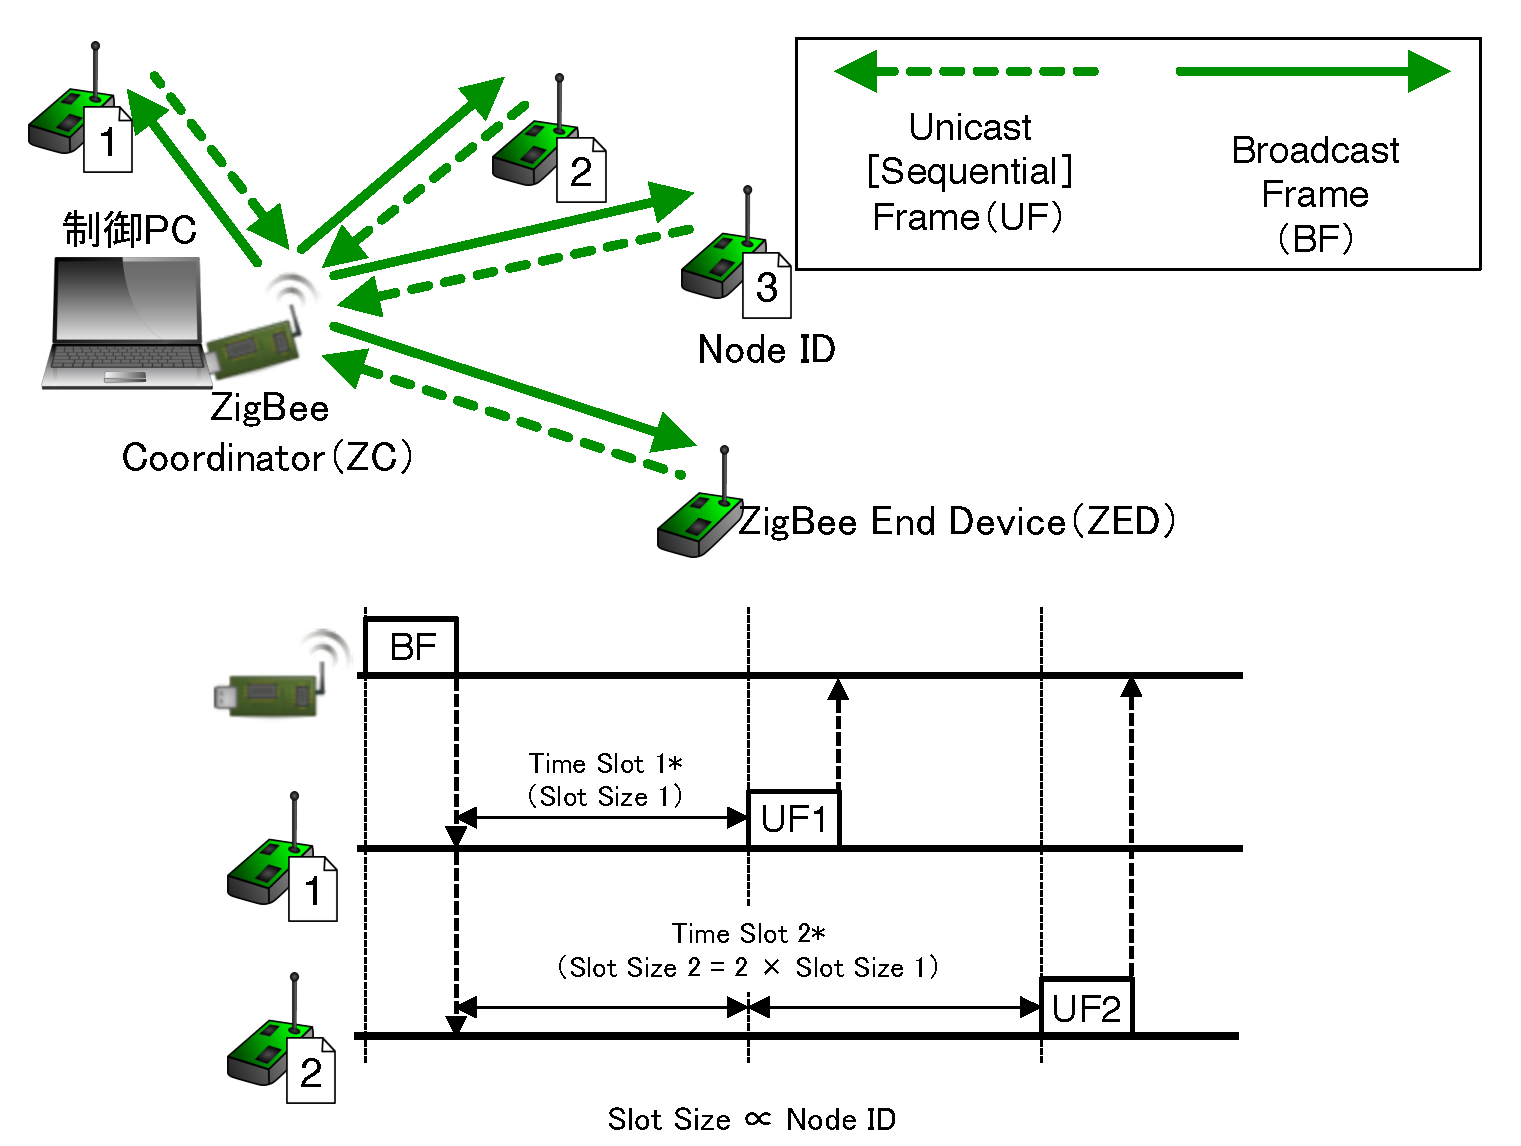
\includegraphics[width=\columnwidth]{figure/aacts_snw.pdf}
 \caption{ZigBeeノードによるデータ収集システム}
 \label{fig:aacts_snw}
\end{figure}

%図\ref{fig:??}にその外観を示す.
%MICAzは
%無線機能,CPU,メモリ等を有したノード部分と各種センサを搭載したセンサ基板部分から構成されるセンサノードであり,
%最大約50mの通信を行うことが可能であり,
%安定動作電圧は3.3V,消費電流は通信時60mA,スリープ時20μAである.
%電源は単三乾電池2本から供給可能である.
%接続基板は
%本システムにおけるZCは,前述したZEDで使用するMICAzと,
%MICAzに対応したCrossbow社のMIB520~\cite{Device:}を用いた.
%I/OインターフェースとしてUSB Aタイプ(オス)を備え,電源はUSB バスを通じてPC から供給する.
%また,出力コンソールとして3色(赤,緑,黄)のLEDを利用できる.
%メス−メスUSB A-Aコネクタ(オス - メス)を用いてMICAz をMIB520 に装着し,制御PCと接続を行った.
%また,MIB520はオンボードでISP(in-system programming)に対応しており,
%シリアル通信及びシステムプログラミングを可能とする.
%但し,

%ノードへのアプリケーション実装は,PCで行った. 
%但し,PCにはTinyOS がインストールされていることが必要条件である.
%TinyOSはオープンソースで開発がされているセンサネットワークノード向けのイベント駆動OSであり,
%これを用いてZED及びZCのZigBee通信アプリケーションを実装した.
%TinyOS上で利用されるイベント駆動型プログラミング言語がnesCであり,C言語の拡張である.

制御PCはDebian GNU/Linuxの動作するdynabook UX/28LWHEMを用いた.
制御アプリケーションはC言語で実装した.
モニターモードの無線LANインタフェースを用い,
libpcapライブラリを利用することで環境中に流れるフレームの
傍受が可能であるため,RTS/CTSフレームのキャプチャを行う.
ソケットライブラリを用いることでRTSフレームの送信,CTSフレームの受信を
可能としている.
%及びZCとの通信を可能としている.

RSSIによるAP選択アルゴリズムにおいても同様に,
モニターモードの無線LANインタフェースを用いて
Radiotapヘッダが付加されたIEEE\,802.11 MACフレームを受信し,
周囲のAPのRSSIを1.5\,秒間収集する.
収集した情報から,RSSIがもっとも大きいAPを選択するものとした.

%ここで,WLANが準拠しているIEEE 802.11で策定されている,
%IEEE 802.11フレーム共通のMACフレーム(参考文献)を\ref{fig:mac_header}に示す.
%スニファにより取得したWLANフレームにおいて,
%MAC(Media Access Control)層で付加されるヘッダを利用する事でWLAN端末接続数の計算は可能である.
%MACヘッダの3〜5ユニット目を抜き出すと,
%Address 1(DA)及びSA,BSSIDがある.
%WLAN端末の通信はAPを介するため,BSSIDとDAまたはSAが一致する筈である.
%APのBSSIDは既知であるため,
%AP1台に対し,APのBSSIDがDAになる場合の相異なるSAは取得可能である.
%その逆も同様に可能である.
%従って,APのBSSIDがDAの場合のSA及び,APのBSSIDがSAの場合のDAの共通部分を取り,
%これをキーとしたテーブルをAP毎に作成する.
%テーブルの行数がAPのWLAN接続台数に等しいため,最も行数の多いAPを選択することが
%AP選択アルゴリズムの決定キーとなる.

%--------------------------------------------------

%----------------------------------------------------------------------
\section{評価}
\label{sec:eval}

提案するAA CTS-Blocking方式の評価について実験及びその結果を示す.
まず,未決定パラメータの最適値を探るため,
%\ref{sec:imple}で述べたTime SlotのSlot Sizeを決定するために,
%電波暗箱内で
データ収集システムの予備実験を行った.
全パラメータ決定後は,AA CTS-Blocking方式がWLANの混雑度に関わらず
効果があることを示すために,
通信時間の違いによる評価を行ったので,報告する.

%評価の流れは書いて欲しい。何のために予備実験をして、
%それからどんな評価(項目のこと)をしているのかの情報が欲しい。

\subsection{予備実験}
\label{ssec:before_exp}

\ref{sec:imple}で述べたTime SlotのSlot Sizeを決定するために,
%電波暗箱内で
データ収集システムの予備実験を行った.
%まず,スロットサイズを決定するために他の電波による干渉がない場所で
%ZigBee通信のみを評価する.
Slot Size決定のためには,他の電波の影響がない環境で
データ収集システムの動作を評価する必要がある.
したがって,電波暗箱(機種名)を評価環境として選択した.
図\ref{fig:nowave_box}に示す通り,電波暗箱内にデータ収集システムを配置した.
ZEDからZCへ送信するデータは,サイズの変化による影響をなくすため
送信元アドレス及びシーケンス番号のみが記録されたダミーデータとした.
サイズはヘッダを含めて18バイトと一定である.
18バイトのデータを送信するのにかかる時間は,
ZigBeeの公称通信速度250\,kbps~\cite{ZigBee04:}から計算すると
0.576\,msとなる.
本システムにおけるSlot Sizeはデータの送信時間に加え,
MICAzの処理時間たる送受反転時間及びガード時間を含めたものを想定している.
採用するSlot SizeではZCのデータ収集率が100\%になるものを選択する必要がある.
ZCは全10台のZEDからダミーデータを収集する.
予備実験では異常値を排除するため,データ収集の試行を200回行うこととする.
\ref{sec:imple}で述べた通り,ZigBeeノード間の通信時間が最大32\,msであり,
データの送信時間が0.576\,msであることを考慮に入れると,
Slot Sizeとして適しているのは1\,ms〜3\,msの場合である.
これについてSlot Size別にデータ収集予備実験を行った.
%なぜSlot Sizeを1~3にしたのか
Packet snifferを用いてエラーパケットの有無を監視し,通信成功台数を測定する.
通信成功台数とは,1回のデータ収集試行でZEDがZCへ送信成功した台数であり
最大値は10台である.
200回試行中のZEDの延べ通信成功台数を
200回試行中ZEDが全て通信成功した台数である2000
で割り通信成功率に変換した.


%・何のために予備実験をやるのか
%・どうやるのか
%・その結果はどうなったのか
%をきちんと分離して書く。1 paragraphは1 topic。
%ZigBeeノードによるデータ収集システムでは
%ZEDからZCへの通信はスケジューリングとしてTDMA方式を利用する際,
%スロットサイズを決める必要がある.
%本システムにおけるスロットサイズはデータの送信時間に加え,
%送受反転時間及びガード時間を含めたものを指す.
%(データの送信時間+システムの処理時間+干渉回避の時間)
%ZEDからZCへ送信するデータは,データサイズの変化による影響をなくすため
%送信元アドレス及びシーケンス番号のみが記録されたダミーデータとした.
%ZCからデータ送信要求を受信すると,各ZEDはあらかじめ割り当てられたスロットに
%おいてダミーデータを送信する.
%サイズはヘッダを含めて18バイトである.
%評価実験においてZEDからZCへ送信するダミーデータの
%フレームを図\ref{fig:dummy_data}に示す.
%18バイトのデータを送信するのにかかる時間は,
%ZigBeeの公称通信速度250\,kbps~\cite{ZigBee04:}から計算すると
%0.576\,msとなる.
%MicaZの送受反転時間及び,ガード時間を含めたスロットサイズを決定するために
%電波暗箱(機種名)内で図\ref{fig:nowave_box}に示す通りにZigBeeノードを配置し通信させた.
%ZCが全10台のZEDからダミーデータを収集する通信を
%1サイクルとし,
%周期200\,msで100サイクル,
%行った.
%スロットサイズ1\,ms〜3\,msの場合について実施した.
%Packet snifferを用いてエラーパケットの有無を監視し,成功率に反映した.
結果,スロットサイズ1\,msでは49.8\%であったのが
2\,msでは99.95\%,3\,msでは99.93\%と100\%に限りなく近い値となった.
スロットサイズは短いほど有利であるため,2\,msとした.

\begin{figure}[bt]
 \centering
 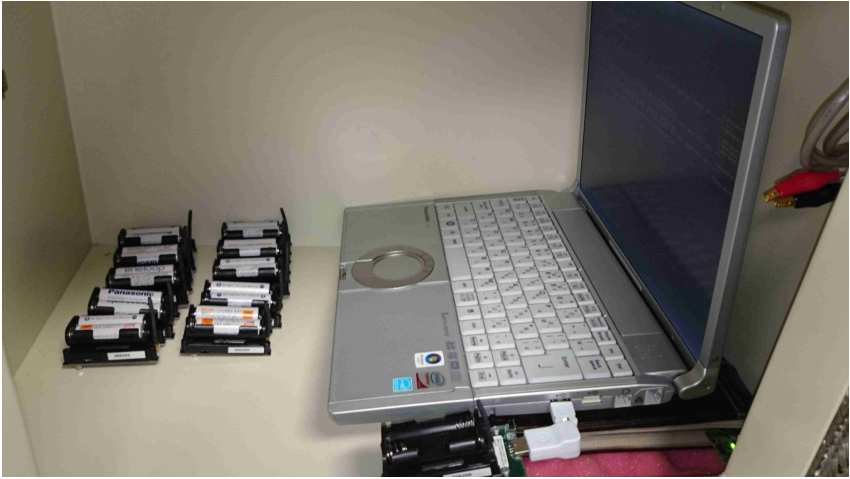
\includegraphics[width=0.3\textwidth]{figure/nowave_box.pdf}
 \caption{電波暗箱内の様子}
 \label{fig:nowave_box}
\end{figure}

\subsection{評価環境}

\begin{figure}[bt]
 \centering
 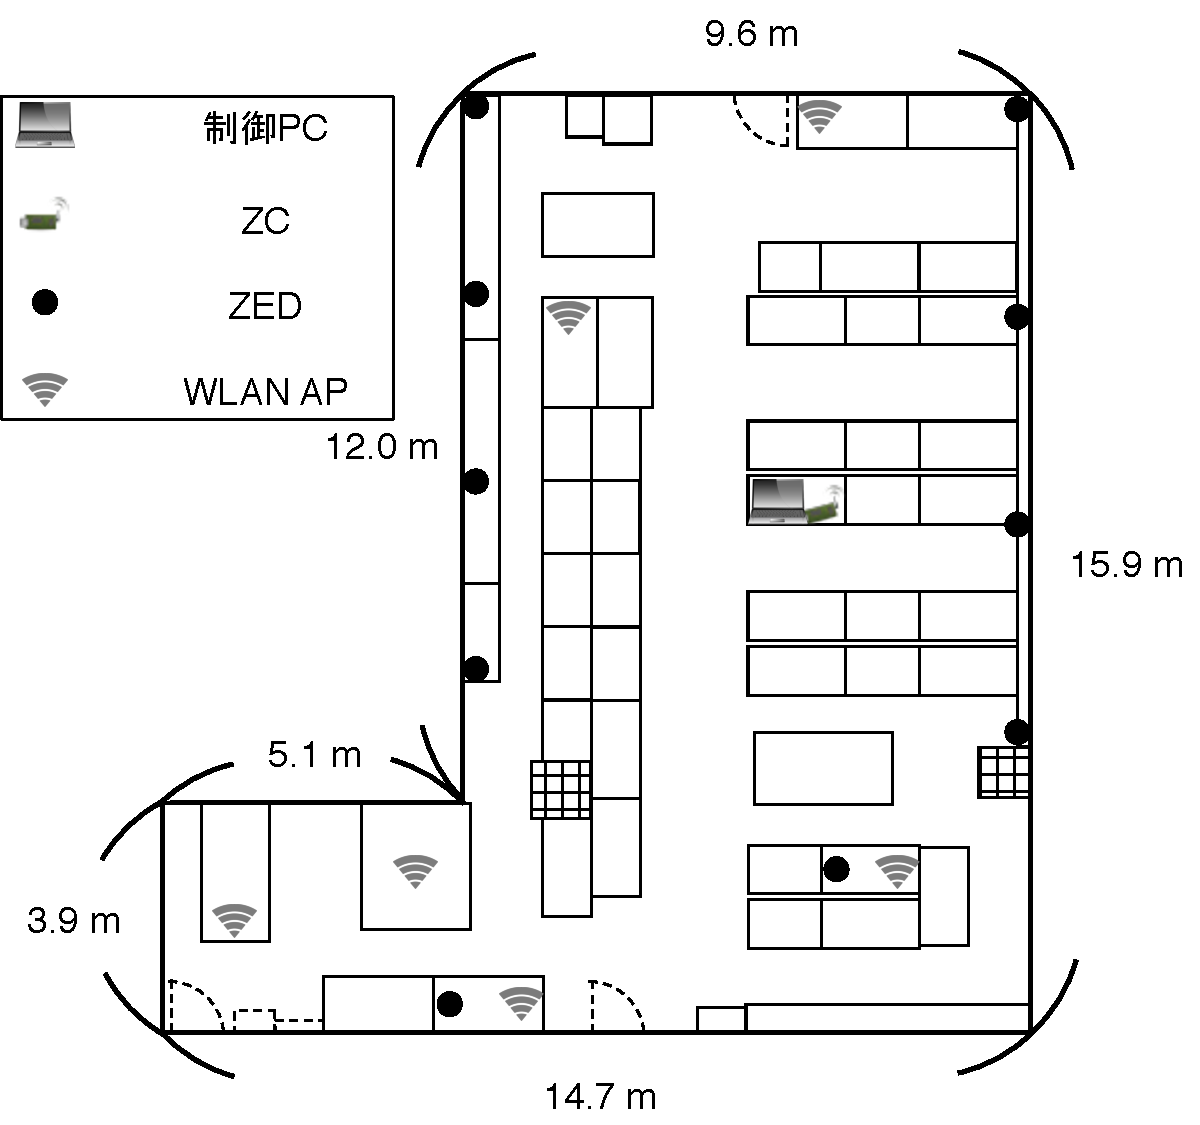
\includegraphics[width=\columnwidth]{figure/fukuda_lab.pdf}
 \caption{実験環境の概略}
 \label{fig:fukuda_lab}
\end{figure}

\ref{sec:aa_cts}で示したAA CTS-Blockingの有効性を検証する評価として,
WLAN通信環境下でのZigBee通信実験を行う.
実験環境として,WLANネットワークが多く存在する筆者の研究室を選択した.
図\ref{fig:fukuda_lab}に実験環境の概略を示す.
研究室内に10台のノードを分散して配置する.
WLANネットワーク側には5台のWLAN端末を用いて通信させ,
約5\,Mbpsの通信負荷を常時発生させた.
通信負荷値の測定にはパケット解析ツールであるWiresharkを用いた.
評価実験の際には,WLANの平均トラフィックが
大幅に変化しないことを確認している.

ZigBee通信時間は
%デバイスの処理時間が遅延する等の外的要因による誤差を考慮し,
\texttt{Duration}フィールドの最大値32\,msを参考に,30\,msを確保した.
本実験では,\figurename~\ref{fig:sequence}で示した(1)〜(7)全体の通信シーケンス,
RTS/CTSフレームを利用して全10台のノードからダミーデータを収集する動作を1サイクルと定義する.
1サイクルの周期は200\,msとし,データ収集を1000サイクル実施した.%データ収集通信の成功率を算出した.
%1000サイクル実施した理由としては,
%これは瞬時値がもたらす評価値への悪影響を平均化により排除するためである.
%例えば瞬間的にWLAN通信の混雑度が変化すると,AA CTS-Blockingの効果も変化すると考えられ,
%意図しない原因によるサイクル毎の通信成功台数のバラ付きが発生する恐れがある.
%従って,評価値の算出は十分多くの試行から平均をとる必要がある.

比較対象として,
(A)~Normal: 何もせずにZigBee通信を行った場合,
(B)~CTS-Blocking: 制御PCから周囲のWLAN端末へ直接CTSを送信した場合,
(C)~AA CTS-Blocking: 制御PCからAPへRTSを送信した場合
のそれぞれについて実験を行う.

評価には2つの軸を設けた.
1つはマクロなZigBee通信成功率を知るために,1000サイクル全体でのZEDの平均通信成功台数を評価する.
通信成功台数は\ref{ssec:before_exp}での定義と同様に,
1回のデータ収集サイクルでZEDがZCへ送信成功した台数であり最大値は10台である.
%1サイクル200\,msのデータ収集通信を1000サイクル実施すれば3分20秒となるため,
%手法の違いによる平均的な通信成功率の評価を行うことができる
%しかし,平均だけではZEDの通信成功台数がサイクル毎にどう変化するのかを知ることができない.
%そこで
もう1つの評価として,ミクロなZigBee通信成功率を知るために,1サイクル毎のZEDの通信成功台数を評価する.
%これを1000サイクル分蓄積させることでヒストグラムとした.
%通信成功台数を示す

%--------------------------------------------------
\subsection{マクロなZigBee通信成功率の比較}
\label{sec:exp_result_all}

\begin{figure}[bt]
 \centering
 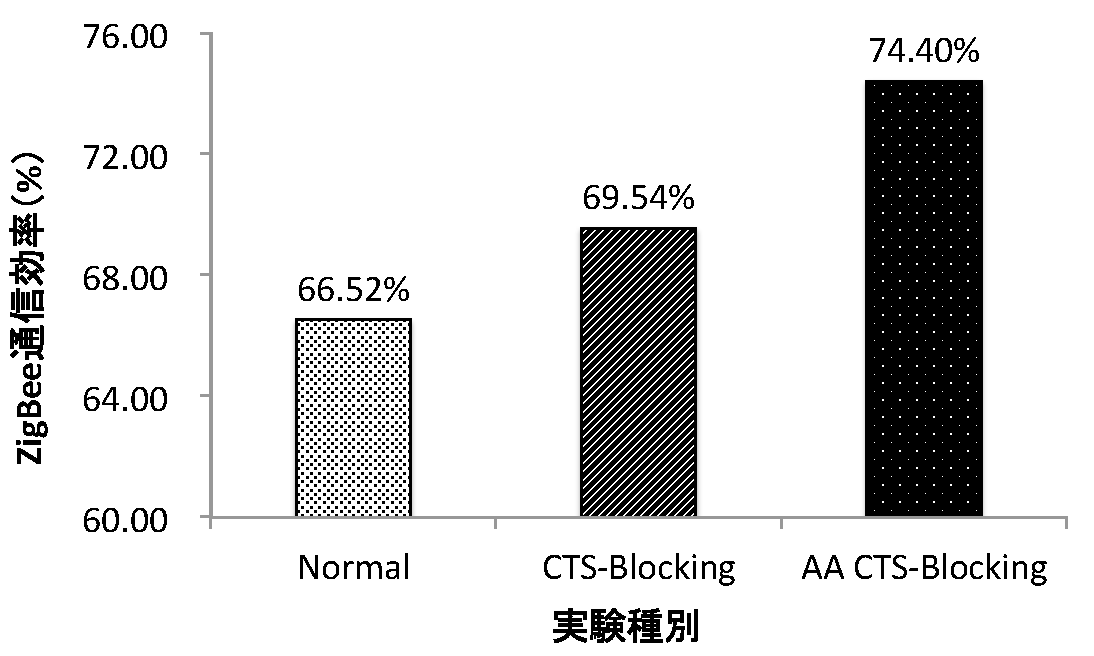
\includegraphics[width=\columnwidth]{figure/eff_all_zigbee.pdf}
 \caption{ZigBee平均通信成功率}
 \label{fig:eff_all_zigbee}
\end{figure}

図\ref{fig:eff_all_zigbee}に,実験種別(A)~Normal,(B)~CTS-Blocking,(C)~AA CTS-Blockingの場合におけるZigBee通信効率を示す.
縦軸のZigBee通信効率は,1000サイクル中のZEDの延べ通信成功台数を最大の総通信成功台数で除した百分率である.
図\ref{fig:eff_all_zigbee}より,以下の2つのことがわかる.
\begin{enumerate}
 \item (C)~AA CTS-Blockingは(A)~Normalに比べ,通信効率が向上している.
(C)~AA CTS-Blockingと(A)~Normalでは約8%程度の差がある.
これは,WLAN通信をブロックしない状況に比べて
AA CTS-Blocking方式によるWLAN通信のブロック効果が大きく出ているためであると考えられる.

 \item (C)~AA CTS-Blockingは(B)~CTS-Blockingに比べ,通信効率が向上している.
(C)~AA CTS-Blockingと(B)~CTS-Blockingでは約5%程度の差がある.
これは,RSSIによるAPの選択アルゴリズムがAA CTS-Blockingによる
周辺のWLAN通信のブロック効果を強めているためであると考えられる.

\end{enumerate}
AA CTS-Blocking方式では制御PCよりも送信電力の高いAPにCTSフレームを送信させることで,
CTS-Blockingの問題点であった隠れ端末問題が改善されてWLANによる干渉の影響を緩和している.

\subsection{ミクロなZigBee通信成功率の比較}
\label{sec:exp_result_part}

\begin{figure}[bt]
 \centering
 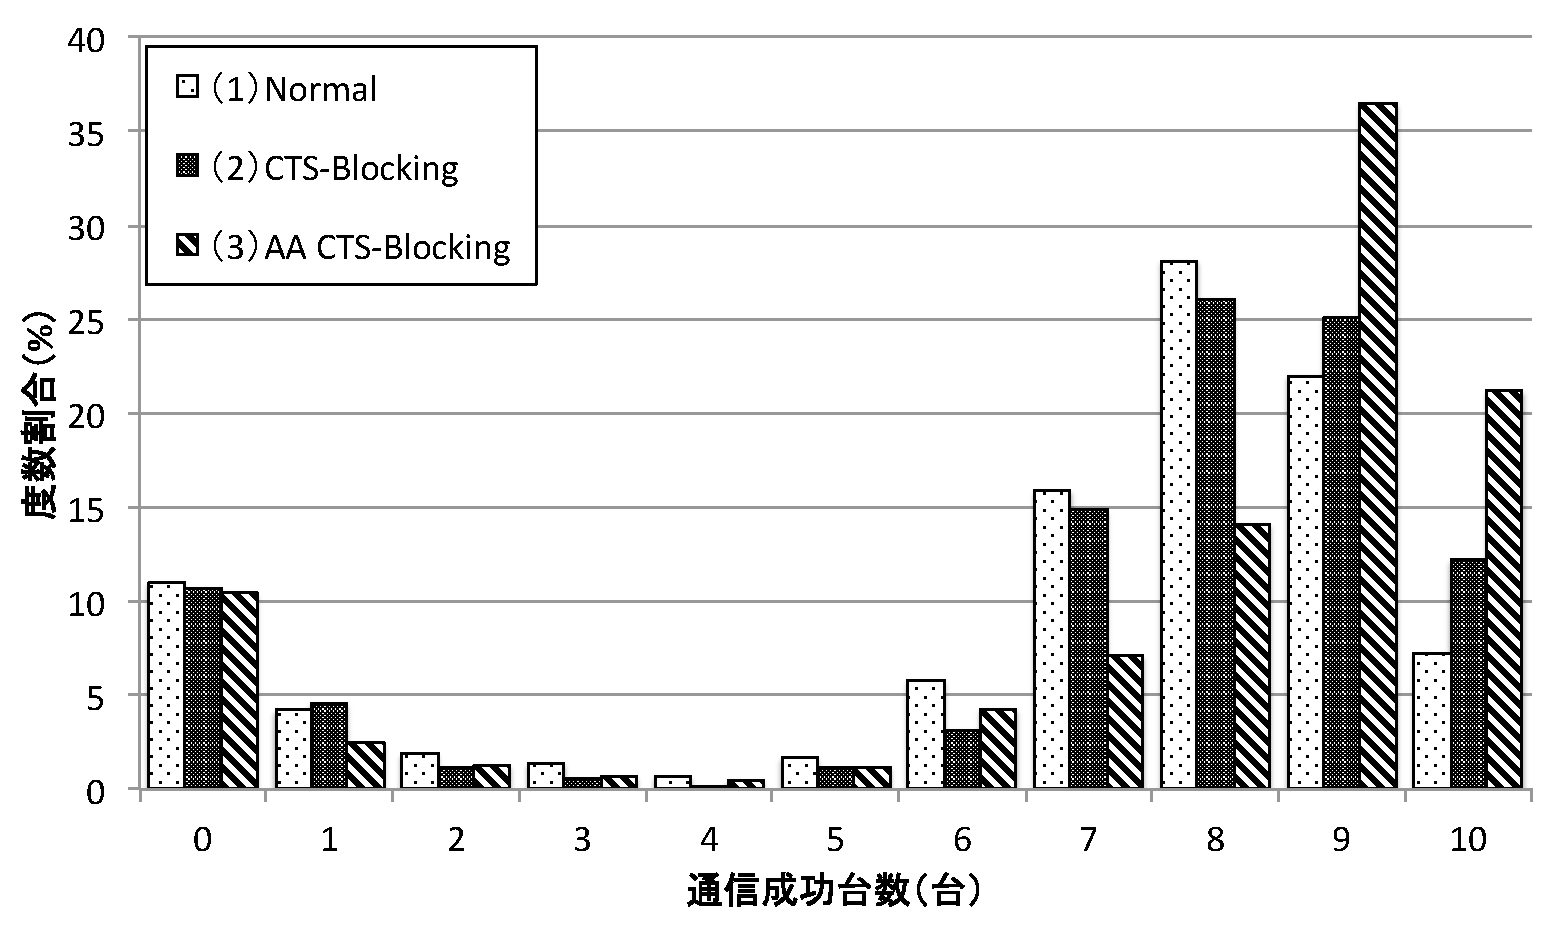
\includegraphics[width=\columnwidth]{figure/eff_one_zigbee.pdf}
 \caption{サイクル毎のZigBee通信成功台数分布}
 \label{fig:eff_one_zigbee}
\end{figure}

\ref{sec:exp_result_all}では,AA CTS-Blocking手法によりマクロなZigBee通信成功率が向上したことを示したが,
平均だけではZEDの通信成功台数が1サイクル毎にどう変化しているかは把握できない.
そこで,局所的なZigBee通信成功率もAA CTS-Blocking手法で向上したことを示す.
図\ref{fig:eff_one_zigbee}に,実験種別(A)~Normal,(B)~CTS-Blocking,(C)~AA CTS-Blockingの場合における
サイクル毎のZigBee通信成功台数分布を示す.
縦軸の度数割合は,1000サイクル中におけるZEDの各通信成功台数のサイクル数を,
1000サイクルで除した百分率である.
図\ref{fig:eff_one_zigbee}より,以下の2つのことがわかる.
%enumerateの中身を変える
\begin{enumerate}
 \item 通信成功台数が5台以下の度数割合は,
 (A)~Normal,(B)~CTS-Blocking, (C)~AA CTS-Blockingであまり変化がない.
これは,AA CTS-Blocking方式を適用してもWLAN通信をブロックする効果をなさないほど
WLAN通信が混雑していた,もしくは
データ収集システムでのZigBeeノード間通信において生じた問題のためであると考えられる.

 \item  (C)~AA CTS-Blockingは(A)~Normal,(B)~CTS-Blockingに比べて
通信成功台数が7台,8台の時の度数割合が大幅に減少しており,
代わりに9台,10台の時の度数割合が大幅に増加している.
これは,(A)~Normal,(B)~CTS-Blockingを利用した場合では
WLAN通信による干渉でZigBeeノード間通信が失敗していた台数分を,
AA CTS-Blocking方式を利用した場合では通信成功台数に変えているためと考えられる.

\end{enumerate}

%------------------------------------------------------------------------enumerateの中へ
%これを見ると,(A)~Normalでは7台の辺りにピークがあり,最大値10の度数は低いことがわかる.
%しかし,(B)~CTS-Blockingではそのピークが右へシフトしていることがわかる.
%(C)~AA CTS-Blockingではその傾向が更に強まっており,最大値の度数も1つのピークとして確認できることから,
%1サイクルあたりの受信メッセージ数は確実に向上している.
%------------------------------------------------------------------------enumerateの中はここまで
AA CTS-Blockingによる通信成功台数の変化は,
1000サイクルの平均といったマクロな視点だけでなく
1サイクル毎といったミクロな視点でも同様に比例して改善し,向上している.

%----------------------------------------------------------------------

\section{おわりに}\label{sec:conclu}

本稿では,WLANとZigBeeの共存に向けたAA CTS Blocking方式を示した.
AA CTS Blockingを利用したデータ収集システムを実装し,実証評価を通
じてAA CTS Blockingの有効性を検証した.
この結果,既存手法よりも通信成功率を5\,\%改善できることを確認した.
今後,通信成功率の更なる向上に向けた
RTS送信先APの選択手法を実装,評価予定である.

%----------------------------------------------------------------------
% 謝辞
%----------------------------------------------------------------------
%\ack
%本研究の一部は,科研費(22300025,25870928) 及び文部科学省「社会システム・
%サービスの最適化のためのIT統合システム構築」(採択課題名: 「社会システム・
%サービス最適化のためのサイバーフィジカルIT統合基盤の研究」)の助成で行わ
%れた.

%----------------------------------------------------------------------
% 参考文献
%----------------------------------------------------------------------
%\bibliographystyle{sieicej}
%\bibliography{bib/IEEEabrv,bib/mystr_IEICE,bib/my,bib/pub}

%----------------------------------------------------------------------
% 参考文献
%----------------------------------------------------------------------
\begin{thebibliography}{99}

\bibitem{Shuaib06:}
K. Shuaib  \textit{et~al.},
``Co-existence of Zigbee and WLAN, A Performance Study", 
Proc. Wireless Telecommunications Symposium, 
Apr. 2006.

\bibitem{Chieh10:}
Chieh-Jan Mike Liang \textit{et~al.},
``Surviving Wi-Fi Interfereence in Low Power ZigBee Networks", 
SenSys’10, 
November 3–5, 2010, 
Zurich, Switzerland.

\bibitem{Hou09:}
J. Hou \textit{et~al.},
``Minimizing 802.11 Interference on Zigbee Medical Sensors", 
Proc. ICST BodyNets,
Apr, 2009.

\bibitem{Huang10:}
J. Huang \textit{et~al.},
``Beyond Co-existence: Exploiting WiFi White Space for ZigBee Performance Assurance", 
Proc. IEEE ICNP,
Oct. 2010.

\bibitem{Kang07:}
MS Kang, \textit{et~al.},
``Adaptive Interference-Aware Multi-Channel Clustering Algorithm in a ZigBee Network in the Presence of WLAN Interference", 
ISWPC '07. 2nd International Symposium on Wireless Pervasive Computing, Fed, 2007.

\bibitem{Murata14:}
村田 亮介 \textit{他},
``無線LANとZigBee間の干渉回避方式の実験評価", 
MoNA, モバイルネットワークとアプリケーション 113(398), 49-53, 
Jan, 2014.

\bibitem{Zhang11:}
X. Zhang \textit{et~al.},
``Enabling Coexistence of Heterogeneous Wireless Systems: Case for ZigBee and WiFi", 
MobiHoc’11, May, 2011.

\bibitem{Shin10:}
SY. Shin \textit{et~al.},
``Active Channel Reservation for Coexistence Mechanism (ACROS) for IEEE 802.15.4 and IEEE 802.11", 
IEICE transactions on communications 93(8), 2082-2087, Aug, 2010.

\bibitem{Huang09:}
ML Huang, \textit{et~al.},
``A WLAN and ZigBee Coexistence Mechanism for Wearable Health Monitoring System", 
ISCIT International Symposium on Communications and Information Technology, Sept, 2009.

\bibitem{Tytgat12:}
L. Tytgat \textit{et~al.},
``Avoiding collisions between IEEE 802.11 and IEEE 802.15.4 through coexistence aware clear channel assessment", 
EURASIP Journal on Wireless Communications and Networking
Apr, 2012.

\bibitem{izumi13:}
和泉 晃 \textit{他},
``ネットワーク側測位における端末固有のRSSIの特性を用いた測位精度向上手法の提案", 
電子情報通信学会技術研究報告. MoMuC, モバイルマルチメディア通信 112(404), 1-6, Mar, 2013. 

\bibitem{Bellardo09:}
J. Bellardo \textit{et~al.},
``802.11 Denial-of-Service Attacks: Real Vulnerabilities and Practical Solutions", 
12th USENIX Security Symposium,
Aug, 2003.

\bibitem{Device:}
J. Bellardo \textit{et~al.},
``XM2110J/MPR2600J/2400J/420/520-MIB Users Manual", 
http://www.xbow.jp/mprmib.pdf

\bibitem{ZigBee04:}
ZB Alliance ,
``ZigBee Overview", \\
http://www.sessionview.com/data/postevent/EU-05/Don-Sturek-8746084.pdf

%---------------------------------------------------------------------------------------------------

%\bibitem{Shin07:}
%SY Shin, \textit{et~al.},
%``Packet Error Rate Analysis of ZigBee Under WLAN and Bluetooth Interferences", 
%IEEE transactions on wireless communications, vol.6, no.8, Aug, 2007.

%---------------------------------------------------------------------------------------------------


\end{thebibliography}

\end{document}
